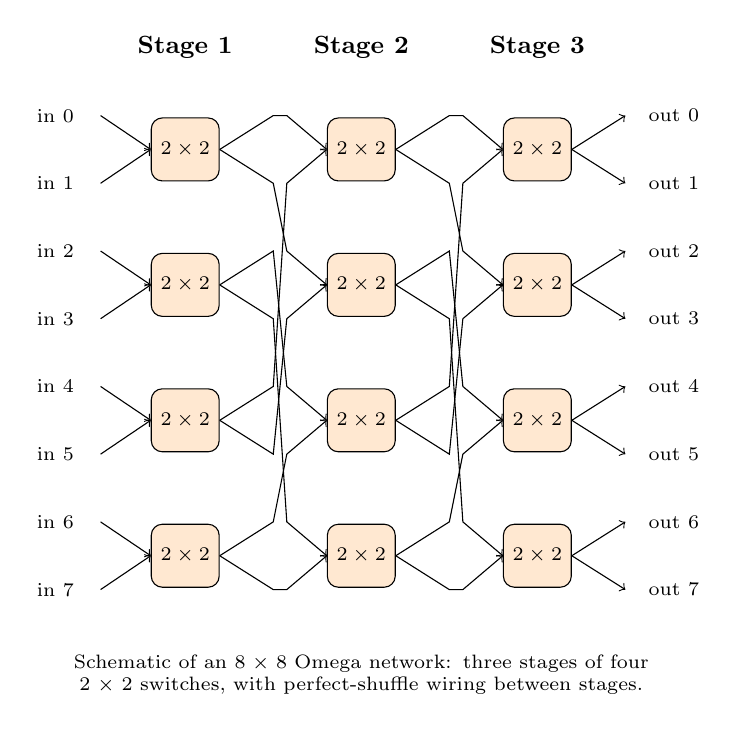
\begin{tikzpicture}[scale=0.86, every node/.style={font=\scriptsize}]
  % Illustrative 8x8 Omega network: three stages, four 2x2 switches per stage.
  \foreach \i in {0,...,7} {
    \node[left] at (0,7-\i) {in \i};
    \node[right] at (8.2,7-\i) {out \i};
  }
  \foreach \s/\x in {1/1.5,2/4.1,3/6.7} {
    \node[font=\small\bfseries] at (\x,8.0) {Stage \s};
    \foreach \j in {0,...,3} {
      \node[draw,rounded corners,fill=orange!18,minimum width=7mm,minimum height=8mm] (sw\s\j) at (\x,6.5-2*\j) {$2\times2$};
    }
  }
  % Inputs to stage 1 (paired adjacent lanes).
  \foreach \i in {0,...,7} {
    \pgfmathtruncatemacro{\j}{int(floor(\i/2))}
    \draw[->] (0.25,7-\i) -- (sw1\j.west);
  }
  % Perfect-shuffle wiring between stages: output lane i goes to input lane (2i mod 7), with 7 fixed.
  \foreach \i in {0,...,7} {
    \pgfmathtruncatemacro{\src}{int(floor(\i/2))}
    \pgfmathtruncatemacro{\k}{ifthenelse(\i==7,7,mod(2*\i,7))}
    \pgfmathtruncatemacro{\j}{int(floor(\k/2))}
    \draw[->] (sw1\src.east) -- (2.8,7-\i) -- (3.0,7-\k) -- (sw2\j.west);
  }
  \foreach \i in {0,...,7} {
    \pgfmathtruncatemacro{\src}{int(floor(\i/2))}
    \pgfmathtruncatemacro{\k}{ifthenelse(\i==7,7,mod(2*\i,7))}
    \pgfmathtruncatemacro{\j}{int(floor(\k/2))}
    \draw[->] (sw2\src.east) -- (5.4,7-\i) -- (5.6,7-\k) -- (sw3\j.west);
  }
  \foreach \i in {0,...,7} {
    \pgfmathtruncatemacro{\j}{int(floor(\i/2))}
    \draw[->] (sw3\j.east) -- (8.0,7-\i);
  }
  \node[align=center,text width=8cm] at (4.1,-1.25) {Schematic of an $8\times8$ Omega network: three stages of four $2\times2$ switches, with perfect-shuffle wiring between stages.};
\end{tikzpicture}
